\subsection{Верхня оцiнка вiдновлюючого спектрального числа для графа кактуса-ланцюжка}

Для довільного зваженого графа кактуса-ланцюжка ${\bf G}$, зображеного на рисунку \ref{Ch1:image}, розглянемо поставлену задачу.
\input{graphs/Сh1}
Нехай елементами ланцюга є графи $F_1,...,F_n$ і для будь-якого $i \in 1...n$:\\ $F_i$ --- цикл $C_m$, де $m\geq4$, $\forall j \in 1...n-1$ пронумеруємо вершини, що належать множині вершин $F_j$ і множині вершин $F_{j+1}$, тобто 
$V(F_j)\cap V(F_{j+1})=j$. Також вершини, у яких степінь дорівнює чотирьом, не є суміжними.


\begin{figure}[H]
    \centering
    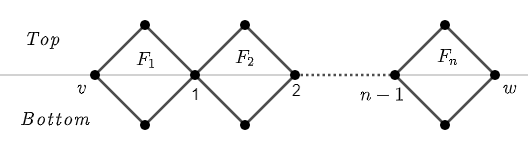
\includegraphics[width=0.7\linewidth]{pictures/Ch4.png}
    \caption{}
    \label{Ch3:image}
\end{figure}
Розташуємо вершини $1,...,n$ і вершини $v, w$ горизонтально у лінію,\\ де $v\in V(F_1)$ і відстань від $v$ до вершини 1 дорівнює двом, $w\in V(F_n)$ і відстань від $w$ до вершини $n$ дорівнює двом. Розіб'ємо $F_1,...,F_n$ на верх і низ(див. рисунок \ref{Ch3:image}). Будемо мати такі дві множини  $VT({G})$ і $VB({G})$, де $VT({G})$ --- множина вершин, що знаходять у верхній області, тобто зверху лінії, і $VB({G})$ --- множина вершин, що знаходять у нижній області, тобто знизу лінії.

Видалимо з графа \textbf{G} вершини з множини $VT({G})$ і отримаємо підграф --- звичайний ланцюг $A_B$, що знаходиться у нижній області, та видалимо з графа \textbf{G} вершини з множини $VB({G})$ і отримаємо підграф --- звичайний ланцюг $A_T$, що знаходиться у верхній області.

Тоді за твердженням 1, ми можемо відновити ваги ребер підграфів $\bf A_B$ і $\bf A_T$, знаючи також підспектри: $\sigma({\bf A_B}-v)$ і $\sigma({\bf A_T}-v)$, де $v$ --- висяча вершина ланцюга $A_B$ і $A_T$.

Отже, такий граф кактус-ланцюжок(див. рисунок \ref{Ch1:image}), можна відновити за чотирма підспектрами:$\sigma({\bf A_B})$, $\sigma({\bf A_B}-v)$, $\sigma({\bf A_T})$, $\sigma({\bf A_T}-v)$, і $Srn({G})\leq4$.